\documentclass[tikz, varwidth=6in]{standalone}

% arara: pdflatex: { interaction: batchmode }
% arara: latexmk: { clean: partial }
\begin{document}

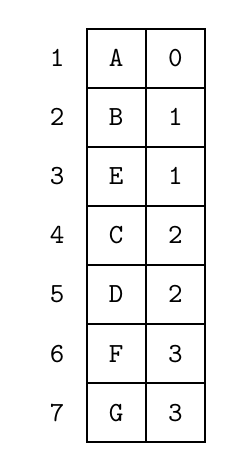
\begin{tikzpicture}[
	thick,
	font=\ttfamily\bfseries,
	minimum/.style={
		minimum width = 0.75cm,
		minimum height = 0.75cm
	},
	box/.style={
		draw,
		rectangle,
		inner sep =+ 0pt,
		minimum
	}
]
\node[box] at (0.00,-0.00) {A};
\node[box] at (0.75,-0.00) {0};
\node[box] at (0.00,-0.75) {B};
\node[box] at (0.75,-0.75) {1};
\node[box] at (0.00,-1.50) {E};
\node[box] at (0.75,-1.50) {1};
\node[box] at (0.00,-2.25) {C};
\node[box] at (0.75,-2.25) {2};
\node[box] at (0.00,-3.00) {D};
\node[box] at (0.75,-3.00) {2};
\node[box] at (0.00,-3.75) {F};
\node[box] at (0.75,-3.75) {3};
\node[box] at (0.00,-4.50) {G};
\node[box] at (0.75,-4.50) {3};

\node[minimum] at (-0.75,-0.00) {1};
\node[minimum] at (-0.75,-0.75) {2};
\node[minimum] at (-0.75,-1.50) {3};
\node[minimum] at (-0.75,-2.25) {4};
\node[minimum] at (-0.75,-3.00) {5};
\node[minimum] at (-0.75,-3.75) {6};
\node[minimum] at (-0.75,-4.50) {7};

\end{tikzpicture}
\end{document}
